%\documentclass[a4paper,12pt,dvipdfm]{report}
\usepackage[brazil]{babel}
%\usepackage[latin1]{inputenc}
\usepackage[utf8]{inputenc}
\usepackage{indentfirst}
\usepackage[pdftex]{color,graphicx}
\usepackage{geometry}
\geometry{top=3cm ,bottom=2cm,left=2.5cm,right=2cm}
%\usepackage{dingbat}

%\usepackage[pdftex]{color,graphicx}
\usepackage{amstext}
\usepackage{amscd}
\usepackage{amsfonts}
\usepackage{float}
\usepackage{textcomp}
\usepackage{amssymb}
%\usepackage{subfigure}
\usepackage{amsmath}
\usepackage{amscd}
%\usepackage{graphics}
%\usepackage{picinpar}
\usepackage{multicol}
\usepackage{multirow}
%\usepackage{epigraph}
%\usepackage[utf8]{inputenc}
%\usepackage{natbib}
%\usepackage{setspace}
\usepackage{mathrsfs}
\usepackage{lscape}
%\usepackage{pdfpages}
\usepackage[normalem]{ulem}
%\usepackage{tikz}
\usepackage[all]{xy}
\usepackage{enumerate}
\usepackage{mathdesign}



%\setcounter{secnumdepth}{5}
%\setcounter{tocdepth}{5}

%\usepackage[brazil]{babel}
%\usepackage[latin1]{inputenc}
%\usepackage[T1]{fontenc}
%\usepackage{indentfirst}
%\usepackage[dvips]{color}
%\usepackage{caption}
%\usepackage{float}
%\usepackage[nottoc]{tocbibind} %inclui referencias no indice.
%\usepackage{enumerate}
%\usepackage{amsmath,amsfonts,amssymb}
%\usepackage{graphicx}
%\usepackage{verbatim}
\usepackage{amsthm}
%\usepackage{natbib}
%\usepackage{subfigure}

%\usepackage{setspace}

\setlength{\parindent}{1.5cm}

\renewcommand{\baselinestretch}{1.5}
\newcommand{\nulo}{\varnothing}
\newcommand{\x}{\times}
%\newcommand{\ital}[1]{\textit{#1}}
%\newcommand{\negr}[1]{\textbf{#1}}
\newcommand{\duascolunas}[2]{\begin{minipage}{7cm} #1 \end{minipage}\hfill\begin{minipage}{7cm} #2 \end{minipage}\\\\} 
\newcommand {\expo}[1]{\exp{\left(#1\right)}}
\newcommand {\expi}[1]{\exp{i\left(#1\right)}}
\newcommand{\arc}[1]{\ensuremath{\overset{\frown}{\raisebox{0pt}[6pt]{#1}}}}


\providecommand{\sin}{} \renewcommand{\sin}{\hspace{2pt}\textrm{sen\hspace{2pt}}}
\providecommand{\tan}{} \renewcommand{\tan}{\hspace{2pt}\textrm{tg\hspace{2pt}}}
\providecommand{\arctan}{} \renewcommand{\arctan}{\hspace{2pt}\textrm{arctg\hspace{2pt}}}
\providecommand{\arcsin}{} \renewcommand{\arcsin}{\hspace{2pt}\textrm{arcsen\hspace{2pt}}}

\theoremstyle{definition}

\newcommand*{\mes}{\ifthenelse{\the\month < 2}{Janeiro}
                  {\ifthenelse{\the\month < 3}{Fevereiro}
                  {\ifthenelse{\the\month < 4}{Março}
                  {\ifthenelse{\the\month < 5}{Abril}
                  {\ifthenelse{\the\month < 6}{Maio}
                  {\ifthenelse{\the\month < 7}{Junho}
                  {\ifthenelse{\the\month < 8}{Julho}
                  {\ifthenelse{\the\month < 9}{Agosto}
                  {\ifthenelse{\the\month < 10}{Stembro}
                  {\ifthenelse{\the\month < 11}{Outubro}
                  {\ifthenelse{\the\month < 12}{Novembro}{Dezembro}}}}}}}}}}}}








\newcommand {\sen}[1]{\sin{\left(#1\right)}}
\newcommand {\cossen}[1]{\cos{\left(#1\right)}}
\newcommand {\tg}[1]{\tan{\left(#1\right)}}
\newcommand {\cotg}[1]{\cot{\left(#1\right)}}
\newcommand {\seca}[1]{\sec{\left(#1\right)}}
\newcommand {\cossec}[1]{\csc{\left(#1\right)}}



\newcommand{\E}{\xi}
\newcommand {\refe}[1]{(\ref{#1})}
%\onehalfspace
%\newcommand {\L}{\mathscr{L}}
\newcommand {\Ima}[1]{\mathrm{Im}{\left[#1\right]}}
\newcommand {\F}{\mathscr{F}}
%\newcommand {\L}{\mathscr{L}}
\newcommand {\om}{\Omega}
\newcommand {\fii}{\varphi}
\newcommand {\lap}{\Delta}
\newcommand {\gra}{\nabla}
\newcommand {\pc}{\vskip 1pc}
\newcommand {\fim}{\nl\rightline{$\square$}\vskip 2pc}
\newcommand {\nl}{\newline}
\newcommand {\cl}{\centerline}
\newcommand {\R}{\mathbb{R}}
\newcommand {\N}{\mathbb{N}}
\newcommand {\Z}{\mathbb{Z}}
\newcommand {\V}{\mathcal{V}^{hp}}
\newcommand {\Q}{\mathbb{Q}}
%\newcommand {\F}{\mathbb{F}}
\newcommand {\G}{\mathbb{G}}
\newcommand {\C}{\mathbb{C}}
\newcommand {\Ss}{\mathbb{S}}
\newcommand {\Ph}{\mathcal{P}_{\!h}}
\newcommand {\B}{\mathcal{B}}
\newcommand {\f}{\mathcal{F}}
\newcommand {\Lh}{\mathcal{L}}
\newcommand {\La}{\Lambda}
\newcommand{\Ri}{\Rightarrow}
\newcommand{\Li}{\Leftarrow}
\newcommand{\lr}{\Longleftrightarrow}
\newcommand{\dis}{\displaystyle}
\newcommand{\lon}{\longrightarrow}
\newcommand{\nin}{/\!\!\!\!\!\in}
%\newcommand {\la}{\lambda}
\newcommand {\al}{\alpha}
\newcommand {\bt}{\beta}
\newcommand {\til}{\widetilde}
\newcommand {\lb}{\linebreak}
\newcommand {\esp}{\hskip 1pc}
\newcommand {\be}{\nl\cl }
\newcommand {\normf}[3]{\Big| \!\! \; \Big|  \dfrac{#1}{#2} \Big| \!\! \; \Big|_{#3}}
\newcommand {\norma}[2] {{\parallel  \! #1 \!  \parallel}_{#2}}
\newcommand {\normp}[1] {{|\!|\!| #1 |\!|\!|}_{\! \Ph}}
\newcommand {\adsum}{\addcontentsline{toc}{subsection}}
\newcommand {\T}{\mathcal{T}}
\newcommand {\ovl}{\overline}
\newcommand {\pref}[1]{(\ref{#1})}
\newcommand {\prcr}[2]{(#1\cup #2)_{\al,L}\rtimes\N}
\newcommand {\tp}[2]{\T(#1\cup #2)}
\newcommand{\mdc}{\text{mdc}}



\newcommand{\funcao}[5]{\begin{array}{cccc}
#1:&\!\!\!#2 & \rightarrow & #3 \\
  &\!\!\! #4 & \mapsto & #5
\end{array}}
\newcommand{\n}{{\bf n}}
\newcommand{\soma}[2]{\displaystyle\sum_{#1}^{#2}}
\newcommand {\flecha}[1] {\stackrel{#1 \rightarrow \infty}\longrightarrow}
\newcommand{\canto}[1]{\begin{flushright} #1 \end{flushright}}
\newcommand{\fd}{\vspace{-0,5cm} \begin{flushright} $\square$ \end{flushright} \vspace{-0,5cm}}
\newcommand{\der}{\partial}
%\newcommand{\sen}{{\rm  \ \! sen}}
\newcommand{\dem}{\hspace{-1.5cm}\textit{Demonstra��o: }}
\newtheorem{teorema}{Teorema}[chapter]

\newtheorem{corolario}[teorema]{Corol\'ario}
\newtheorem{lema}[teorema]{Lema}
\newtheorem{proposicao}[teorema]{Proposi\c{c}\~ao}

%\newtheorem{lema}{Lema}[chapter]
%\newtheorem{corolario}{Corol�rio}[chapter]
%\newtheorem{proposicao}{Proposi��o}[chapter]

\newtheorem{definicao}{Defini\c{c}\~{a}o}[section]
\newtheorem{propriedade}{Propriedades}[section]
\newtheorem*{obs}{Observa\c{c}\~{a}o}
\newtheorem{ex}{Exemplo}[section]
\newtheorem*{solucao}{Solu\c{c}\~{a}o}
\newtheorem*{demo}{Demonstra\c{c}\~{a}o}
%\everymath{\displaystyle}
\setcounter{secnumdepth}{3}
%\voffset 3.8cm
\begin{document}
\DeclareGraphicsExtensions{.pdf,.png,.mps,.jpg}

\chapter{Evolução e Cooperação}

As interações humanas em sua maioria são comparável com algum tipo de jogo, mais especificamente com o jogo dilema do prisioneiro. Neste capítulo estudaremos apenas este jogo. 

Afim de melhorarmos nossa compreensão do jogo, usaremos uma matriz $R$ que mostra apenas o ganho individual do jogador $j_i$, a notação $C$ para coopera e $N$ para não coopera

\begin{equation}\nonumber
R=\bordermatrix{
&C&N\cr
C&a& b \cr
N &c&d
}
\end{equation}\vspace{0.1cm}

Então, se os indivíduos estão interagindo usando a estratégia $(C,C)=$ (coopera, coopera), então ambos obtém como recompensa o valor $a$. Se estão interagindo usando a estratégia $(N,N)=$ (não coopera, não coopera), então ambos obtém como recompensa o valor $d$. Se um usa a estratégia $C =$ (coopera) e o outro $N=$ (não coopera) na interação, então o primeiro obtém $b$ como recompensa e segundo, $c$. E para simplificar a notação, representaremos $R$ apenas por 

\begin{equation}\nonumber
R=\begin{pmatrix}
a & b\\c & d
\end{pmatrix}
\end{equation}\vspace{0.1cm}

Os valores das recompensas devem seguir as seguinte regras $b<d<a<c$ para que o jogo continue sendo um dilema do prisioneiro, ou seja, o jogador $j_i$ que cooperar com quem não coopera tem a pior recompensa, seguido pela recompensa por não cooperar com quem não coopera, que por sua vez é menor que a recompensa de quem coopera com quem coopera e a melhor recompensa é pra quem não coopera com quem coopera.

Usaremos os seguintes valores de recompensa, que chamaremos convenientemente de pontos.

\begin{equation}\nonumber
R=\begin{pmatrix}
3 & 0\\5 & 1
\end{pmatrix}
\end{equation}\vspace{0.1cm}

Vimos no capítulo anterior que o equilíbrio de Nash para esse jogo é a estrategia pura $\textbf{e}=(N,N)=$ (não coopera, não coopera), ambos acusam o outro e recebem 1 pondo por isso. 

\section{Jogos Consecutivos}

Suponhamos que os jogadores repitam o mesmo jogo e somem os pontos obtidos. Vejamos alguns exemplos onde um jogador $j_i$ que nunca coopera joga 10 jogos com um jogador $j_n$ com jogadas aleatórias.

\begin{table}[H]
\centering
\begin{tabular}{|c|c|c|c|c|c|c|c|c|c|c|c|c|}\hline
\multirow{2}{*}{$j_i$} & Jogadas & N & N & N & N & N & N & N & N &	N &	N & Total\\\cline{2-12}
 & Pontos & 5 & 1 & 1 & 1 & 1 & 5 & 5 & 1 & 5 & 1 & 26\\\hline\hline
\multirow{2}{*}{$j_n$} & Jogadas & C & N & N & N & N & C & C & N &	C &	N & Total\\\cline{2-12}
 & Pontos & 0 & 1 & 1 & 1 & 1 & 0 & 0 & 1 & 0 & 1 & 6\\\hline
\end{tabular}
\caption{Saldo de pontos do jogador $j_i$ jogando com um jogador $j_n$ com jogadas aleatórias.}
\label{tab1}
\end{table}

\begin{figure}[H]
\centering
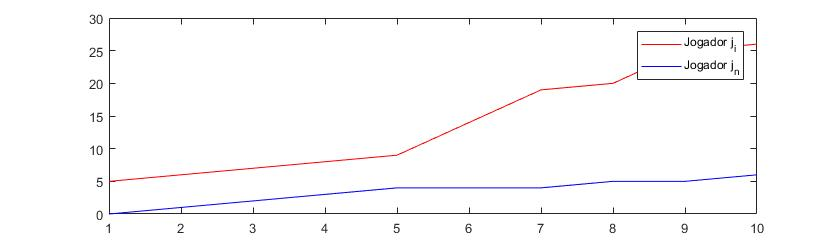
\includegraphics[width=14cm]{imagens/graf1.jpg}
\caption{Soma de pontos dos jogadores $j_i$ e $j_n$.}
\label{fig1}
\end{figure}

\begin{table}[H]
\centering
\begin{tabular}{|c|c|c|c|c|c|c|c|c|c|c|c|c|}\hline
\multirow{2}{*}{$j_i$} & Jogadas & N & N & N & N & N & N & N & N &	N &	N & Total\\\cline{2-12}
 & Pontos & 5 & 1 & 1 & 1 & 1 & 1 & 5 & 1 & 1 & 1 & 18\\\hline\hline
\multirow{2}{*}{$j_n$} & Jogadas & C & N & N & N & N & N & C & N &	N &	N & Total\\\cline{2-12}
 & Pontos & 0 & 1 & 1 & 1 & 1 & 1 & 0 & 1 & 1 & 1 & 8\\\hline
\end{tabular}
\caption{Saldo de pontos do jogador $j_i$ jogando com um jogador $j_n$ com jogadas aleatórias.}
\label{tab2}
\end{table}

\begin{figure}[H]
\centering
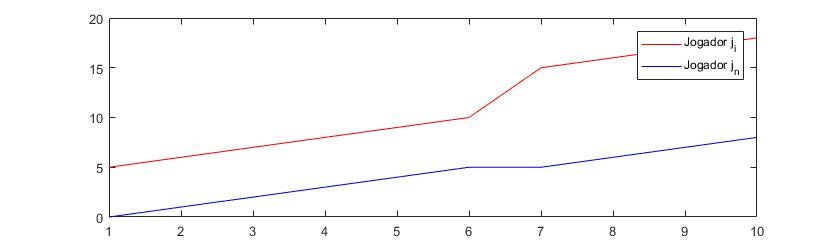
\includegraphics[width=14cm]{imagens/graf2.jpg}
\caption{Soma de pontos dos jogadores $j_i$ e $j_n$.}
\label{fig2}
\end{figure}

Notemos que, apesar de o jogador $j_i$ sempre vencer, o jogador $j_n$ fica com saldo de pontos mais próximo de $j_i$ quando coopera menos vezes, vejamos agora o mesmo jogador $j_i$ jogando com outro jogador $j_n$ que também não coopera.

\begin{table}[H]
\centering
\begin{tabular}{|c|c|c|c|c|c|c|c|c|c|c|c|c|}\hline
\multirow{2}{*}{$j_i$} & Jogadas & N & N & N & N & N & N & N & N &	N &	N & Total\\\cline{2-12}
 & Pontos & 1 & 1 & 1 & 1 & 1 & 1 & 1 & 1 & 1 & 1 & 10\\\hline\hline
\multirow{2}{*}{$j_n$} & Jogadas & N & N & N & N & N & N & N & N &	N &	N & Total\\\cline{2-12}
 & Pontos & 1 & 1 & 1 & 1 & 1 & 1 & 1 & 1 & 1 & 1 & 10\\\hline
\end{tabular}
\caption{Saldo de pontos do jogador $j_i$ jogando com um jogador $j_n$ que nunca coopera.}
\label{tab3}
\end{table}

\begin{figure}[H]
\centering
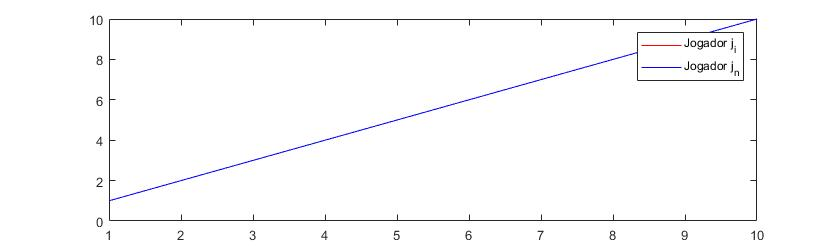
\includegraphics[width=14cm]{imagens/graf3.jpg}
\caption{Soma de pontos dos jogadores $j_i$ e $j_n$.}
\label{fig3}
\end{figure}

Isso já era esperado porque não cooperar é um equilíbrio de Nash no jogo único. Mas vejamos um jogo curioso, onde dois jogadores cooperam entre si.

\begin{table}[H]
\centering
\begin{tabular}{|c|c|c|c|c|c|c|c|c|c|c|c|c|}\hline
\multirow{2}{*}{$j_i$} & Jogadas & C & C & C & C & C & C & C & C & C & C & Total\\\cline{2-12}
 & Pontos & 3 & 3 & 3 & 3 & 3 & 3 & 3 & 3 & 3 & 3 & 30\\\hline\hline
\multirow{2}{*}{$j_n$} & Jogadas & C & C & C & C & C & C & C & C & C & C & Total\\\cline{2-12}
 & Pontos & 3 & 3 & 3 & 3 & 3 & 3 & 3 & 3 & 3 & 3 & 30\\\hline
\end{tabular}
\caption{Saldo de pontos de dois jogadores que sempre cooperam.}
\label{tab4}
\end{table}

\begin{figure}[H]
\centering
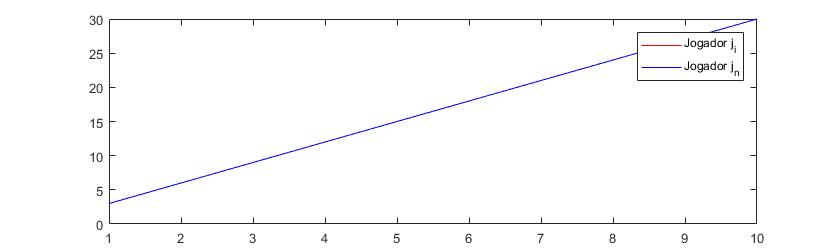
\includegraphics[width=14cm]{imagens/graf4.jpg}
\caption{Soma de pontos dos jogadores $j_i$ e $j_n$.}
\label{fig4}
\end{figure}

Apesar de os ganhos serem garantidamente maiores quando ambos coopera, assim que um descobre que o outro está cooperando ele é tentado a não cooperar e maximizar sua recompensa, e por mais que um deles insista em continuar cooperando, as perdas o força a não cooperar também.

Uma estratégia que evita essa perda, é a \textit{olho por olho}, onde o jogador começa cooperando e depois repete a jogada do outro jogador no jogo anterior. Essa estratégia deixa o jogador o mais próximo possível do vencedor, mas não o supera, alcança no máximo um empate. Veja alguns exemplos: 

\begin{table}[H]
\centering
\begin{tabular}{|c|c|c|c|c|c|c|c|c|c|c|c|c|}\hline
\multirow{2}{*}{$j_i$} & Jogadas & N & C & C & N & N & N & C & N &	C &	N & Total\\\cline{2-12}
 & Pontos & 5 & 0 & 3 & 5 & 1 & 1 & 0 & 5 & 0 & 5 & 25\\\hline\hline
\multirow{2}{*}{Olho por olho} & Jogadas & C & N & C & C & N & N & N & C &	N &	C & Total\\\cline{2-12}
 & Pontos & 0 & 5 & 3 & 0 & 1 & 1 & 5 & 0 & 5 & 0 & 20\\\hline
\end{tabular}
\caption{Saldo de pontos do jogador $j_i$, com jogadas aleatórias, jogando com um jogador \textit{olho por olho}.}
\label{tab5}
\end{table}

\begin{figure}[H]
\centering
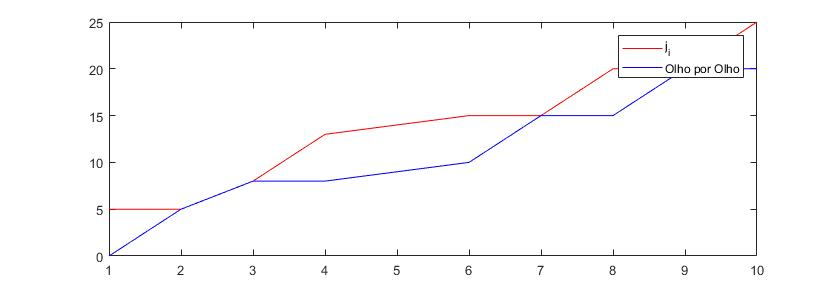
\includegraphics[width=14cm]{imagens/graf5.jpg}
\caption{Soma de pontos dos jogadores $j_i$ e \textit{olho por olho}.}
\label{fig5}
\end{figure}

\begin{table}[H]
\centering
\begin{tabular}{|c|c|c|c|c|c|c|c|c|c|c|c|c|}\hline
\multirow{2}{*}{$j_i$} & Jogadas & N & C & N & C & N & C & N & C &	C &	C & Total\\\cline{2-12}
 & Pontos & 5 & 0 & 5 & 0 & 5 & 0 & 5 & 0 & 3 & 3 & 26\\\hline\hline
\multirow{2}{*}{Olho por olho} & Jogadas & C & N & C & N & C & N & C & N &	C &	C & Total\\\cline{2-12}
 & Pontos & 0 & 5 & 0 & 5 & 0 & 5 & 0 & 5 & 3 & 3 & 26\\\hline
\end{tabular}
\caption{Saldo de pontos do jogador $j_i$, com jogadas aleatórias, jogando com um jogador \textit{olho por olho}.}
\label{tab6}
\end{table}

\begin{figure}[H]
\centering
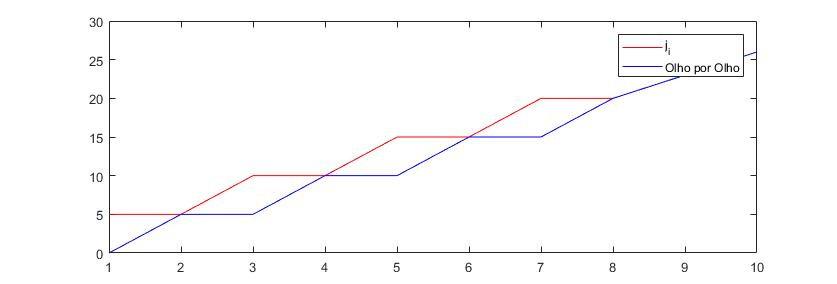
\includegraphics[width=14cm]{imagens/graf6.jpg}
\caption{Soma de pontos dos jogadores $j_i$ e \textit{olho por olho}.}
\label{fig6}
\end{figure}

\begin{table}[H]
\centering
\begin{tabular}{|c|c|c|c|c|c|c|c|c|c|c|c|c|}\hline
\multirow{2}{*}{$j_i$} & Jogadas & N & N & N & N & N & N & N & N &	N &	N & Total\\\cline{2-12}
 & Pontos & 5 & 1 & 1 & 1 & 1 & 1 & 1 & 1 & 1 & 1 & 14\\\hline\hline
\multirow{2}{*}{Olho por olho} & Jogadas & C & N & N & N & N & N & N & N &	N &	N & Total\\\cline{2-12}
 & Pontos & 0 & 1 & 1 & 1 & 1 & 1 & 1 & 1 & 1 & 1 & 9\\\hline
\end{tabular}
\caption{Saldo de pontos do jogador $j_i$, com que nunca coopera, jogando com um jogador \textit{olho por olho}.}
\label{tab7}
\end{table}

\begin{figure}[H]
\centering
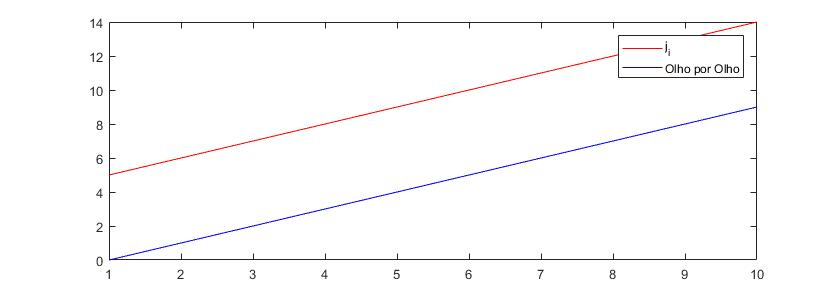
\includegraphics[width=14cm]{imagens/graf7.jpg}
\caption{Soma de pontos dos jogadores $j_i$ e \textit{olho por olho}.}
\label{fig7}
\end{figure}

\begin{table}[H]
\centering
\begin{tabular}{|c|c|c|c|c|c|c|c|c|c|c|c|c|}\hline
\multirow{2}{*}{Olho por olho} & Jogadas & C & C & C & C & C & C & C & C & C & C & Total\\\cline{2-12}
 & Pontos & 3 & 3 & 3 & 3 & 3 & 3 & 3 & 3 & 3 & 3 & 30\\\hline\hline
\multirow{2}{*}{Olho por olho} & Jogadas & C & C & C & C & C & C & C & C & C & C & Total\\\cline{2-12}
 & Pontos & 3 & 3 & 3 & 3 & 3 & 3 & 3 & 3 & 3 & 3 & 30\\\hline
\end{tabular}
\caption{Saldo de pontos de dois jogadores \textit{olho por olho} jogando entre si.}
\label{tab8}
\end{table}

\begin{figure}[H]
\centering
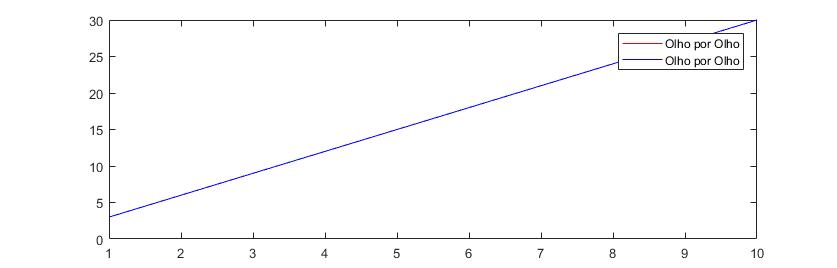
\includegraphics[width=14cm]{imagens/graf8.jpg}
\caption{Soma de pontos dos jogadores \textit{olho por olho}.}
\label{fig8}
\end{figure}

A estratégia \textit{olho por olho} tem uma vantagem sobre a não coopera nunca, que é a de maximizar os ganho quando joga com outro jogador com a mesma estratégia, enquanto o não que coopera nunca, em 10 jogadas ganhou apenas 10 pontos contra um opositor com a mesma estratégia, o olho por olho ganhou 30 pontos.

A limitação da estratégia olho por olho, como veremos a seguir, é que o jogador só pode retalhar o outro jogador na jogada seguinte, se os jogos forem sempre com o mesmo jogador. Numa população de indivíduos onde eles jogam entre si, essa estratégia não é viável.

\subsection{Coeficiente de Reputação}

Em um grupo ou população de jogadores, podemos fazer jogos onde pegamos aleatoriamente dois jogadores e fazemos o jogo entre eles, isso faz com que o próximo jogo de cada jogador, raramente seja com o mesmo jogador anterior, então para guardar um histórico de cada jogador, associaremos a cada um deles um coeficiente $p\in[0,1]$, que chamaremos de coeficiente de reputação, ou apenas a reputação do jogador $j_i$. Esse coeficiente será a probabilidade desse indivíduo cooperar no jogo, ou seja, quem tem uma reputação maior, tem maior chance de cooperar. 

Os jogadores na hora da partida vão escolher sua estratégia baseada na sua reputação e na do seu oponente. A probabilidade do jogador $j_i$ cooperar vai ser a média aritmética da sua reputação e a reputação do outro jogador. O gráfico \ref{fig11} a seguir, mostra a quantidade de pontos que cada jogador ganha em função da sua reputação, numa simulação\footnote{A simulação foi feita no MATLAB e o algorítimo está anexado ao trabalho, no Apêndice 1} onde dois jogadores são selecionados aleatoriamente para jogar $10^5$ vezes, de uma população de 100 indivíduos com reputação linearmente distribuída de 0 a 1, e seus pontos são acumulados.

\begin{figure}[H]
\centering
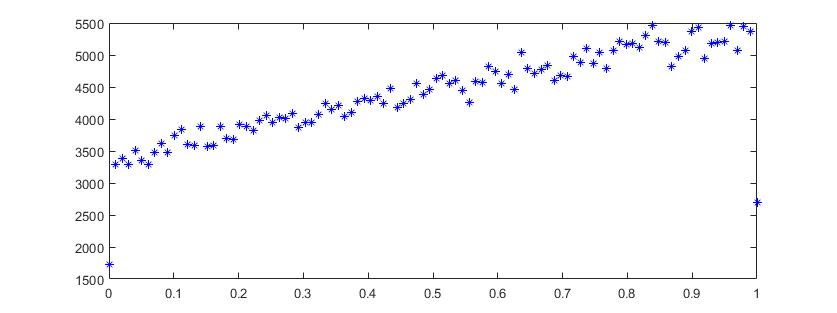
\includegraphics[width=14cm]{imagens/graf11.jpg}
\caption{Quantidade de pontos em função da reputação dos jogadores.}
\label{fig11}
\end{figure}

O jogador com maior reputação acumula mais pontos, e essa diferença fica mais visível quando usamos uma média aritmética ponderada, onde cada jogador dá mais peso para a reputação do seu adversário. Veja os gráficos a seguir onde o jogador dá peso 2 para reputação do adversário e peso 1 pra sua (gráfico \ref{fig12}), e peso 3 para seu adversário e 1 para a sua (gráfico \ref{fig13}).

\begin{figure}[H]
\centering
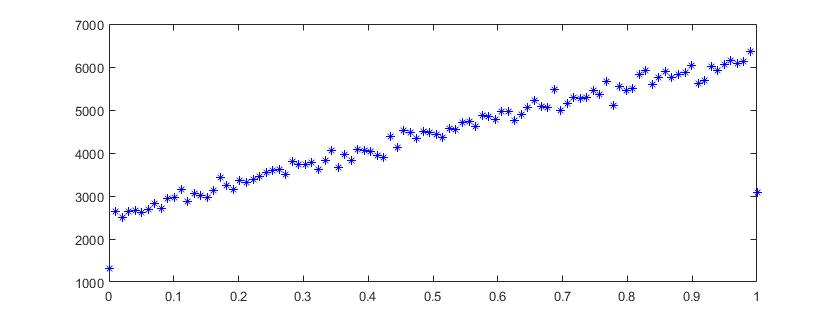
\includegraphics[width=14cm]{imagens/graf12.jpg}
\caption{Quantidade de pontos em função da reputação dos jogadores.}
\label{fig12}
\end{figure}

\begin{figure}[H]
\centering
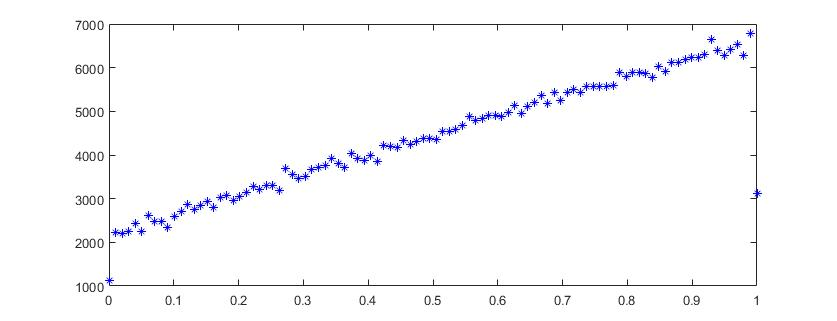
\includegraphics[width=14cm]{imagens/graf13.jpg}
\caption{Quantidade de pontos em função da reputação dos jogadores.}
\label{fig13}
\end{figure}

É possível ver que o indivíduo que tem reputação 0 tem pouco pontos, isso se dá porque os outros jogadores quando feito a média ficam com uma probabilidade baixa de cooperar com ele. O jogador com reputação 1 também fica com pouco pontos, e isso 
é resultado de ele cooperar sempre.

\section{Jogos Evolutivos}

Suponhamos que os jogadores possa aprender com suas jogadas de jogos anteriores e as jogadas dos outros jogadores, ou seja, que eles possam evoluir suas estratégias. Definiremos uma nova forma de pontuação, a matriz de recompensas continuará a mesma, mas os pontos passarão a ser número de indivíduos gerados na população. Inicialmente vamos dividir a população em dois grupos, o grupo dos que cooperam sempre $A$ e o dos que nunca cooperam $B$, eles vão jogar entre si, e o resultado de cada jogo, será o numero de indivíduo que aquele grupo ganhará ou gerará, ou seja, se ambos os indivíduos selecionados forem do grupo $A$, então o jogo será $(C,C)$ onde cada um ganha 3 pontos que significa mais 6 jogadores para o seu grupo $A$, se ambos forem do grupo $B$ o jogo será $(N,N)$ e por consequência cada um ganhará 1 ponto que resulta em 2 indivíduos para o grupo $B$, e por fim se os dois selecionados forem um de cada grupo, o que coopera não ganha ponto portanto seu grupo $A$ não ganha indivíduo e o que não coopera ganha 5 indivíduos para seu grupo $B$; e então mediremos qual grupo cresce mais.

O gráfico \ref{fig9} mostra uma simulação\footnote{A simulação foi feita no MATLAB e o algorítimo está anexado ao trabalho, no Apêndice 2} de uma população de 1000 indivíduos em que 50\% deles cooperam sempre, grupo $A$ e os outros 50\% nunca cooperam, grupo $B$; dois indivíduos serão selecionados aleatoriamente para jogar um com o outro, e os indivíduos gerados a cada jogo será somado ao seu respectivo grupo, ao repetirmos esse processo calcularemos o percentual de cada grupo e aplicaremos esse percentual sobre a população inicial, corrigido o percentual de indivíduos de cada grupo pelo resultado do jogo. Chamaremos essas novas população de novas gerações gerações.

\begin{figure}[H]
\centering
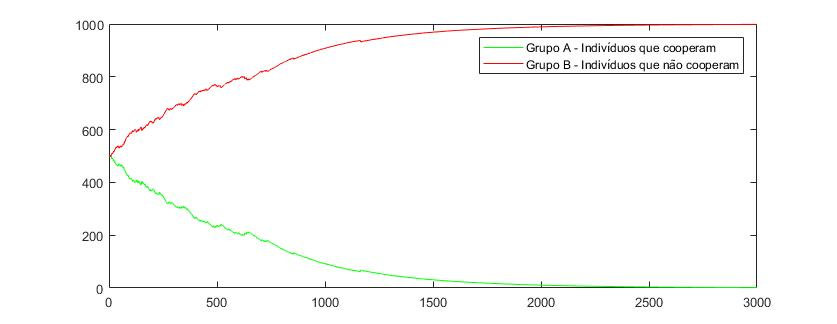
\includegraphics[width=14cm]{imagens/graf9.jpg}
\caption{Evolução da não cooperação em 3000 gerações.}
\label{fig9}
\end{figure}

Não cooperar é a melhor estratégia sempre, esse resultado é obtido independente do percentual inicial da população, como mostra o gráfico \ref{fig10}, de uma simulação com uma população inicial com percentual de 90\% de indivíduos que cooperam e apenas 10\% de não cooperam, e ainda assim a não cooperação prevalece.

\begin{figure}[H]
\centering
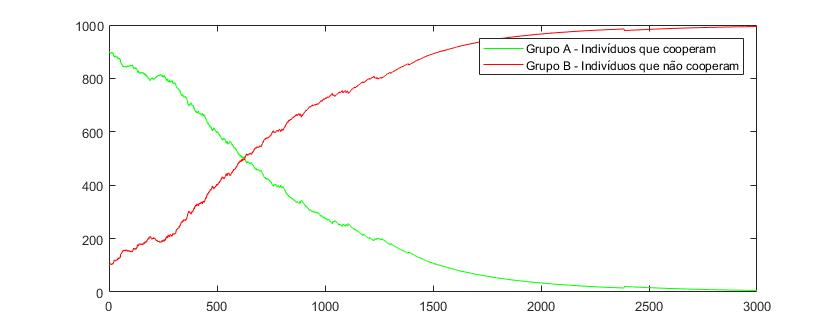
\includegraphics[width=14cm]{imagens/graf10.jpg}
\caption{Evolução da não cooperação em 3000 gerações.}
\label{fig10}
\end{figure}

\subsection{Evolução da Cooperação}

Vamos criar uma população com 100 indivíduos e terá dois coeficientes $p$ e $q$ associados a cada um dele, o coeficiente $p$ será sua reputação, que inicialmente será um número aleatório no intervalo $[0,1]$ e o coeficiente $q$, que chamaremos perfil do jogador, será o peso que esse jogador dará a reputação do seu oponente, também no intervalo $[0,1]$. 

Na primeira etapa da simulação\footnote{A simulação foi feita no MATLAB e o algorítimo está anexado ao trabalho, no Apêndice 3}, será ser escolhido aleatoriamente dois jogadores e eles jogarão usando uma probabilidade de cooperar baseada na média aritmética ponderada entre a reputação dele e a do adversário, usando o seu perfil como peso, seja $p_i$ e $p_n$ a reputação do jogador $j_i$ e $j_n$, e $q_i$ o perfil do jogador $j_i$, então a probabilidade do jogador $j_i$ cooperar nessa jogada contra o jogador $j_n$ será $(1-q_i)p_i+q_ip_n$. Vai ser executado 5000 jogos e depois somados seus pontos, através da matriz $R$ e as reputações serão ajustadas obedecendo a seguinte matriz

\begin{equation}\nonumber
P=\begin{pmatrix}
0.5 & 1\\-1 & 0
\end{pmatrix}
\end{equation}\vspace{0.1cm} 

Onde se o jogador cooperou com outro que cooperou, cada um ganha $0.5$ ponto de reputação, se ambos não cooperam um com o outro então ambos não ganham reputação e se um coopera e o outro não, o que cooperou ganha $1$ ponto de reputação e o que não cooperou perde $1$ ponto.

Na segunda etapa, os perfis da população inicial serão atualizados, os perfis não serão distribuídos aleatoriamente com distribuição normal entre 0 e 1, e sim obedecendo que mais se aproxima ao gráfico que relaciona pontos com perfil, ou seja, os perfis que geraram mais pontos para seus jogadores, serão mais replicados; como se os jogadores estivessem aprendendo com os que têm melhores resultados. E isso vai se repetir 1000 etapas.

O que podemos observar foi que reputação quando maior a reputação do indivíduo, maior a sua quantidade de pontos, veja o gráfico \ref{fig14} que relaciona a reputação de cada jogador com seus pontos acumulados, e traça uma reta que mais se ajusta aos pontos.

\begin{figure}[H]
\centering
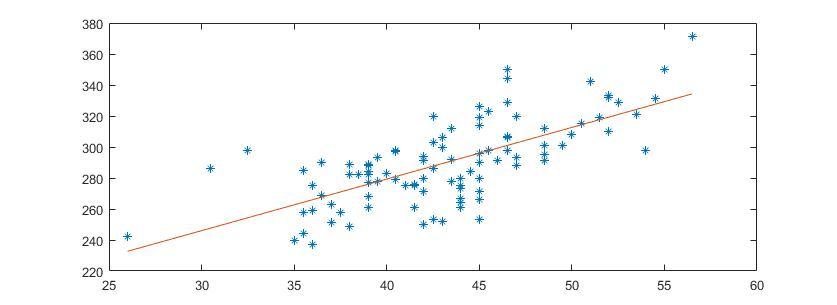
\includegraphics[width=14cm]{imagens/graf14.jpg}
\caption{Pontos acumulados em relação a reputação e o ajuste dos pontos por uma reta}
\label{fig14}
\end{figure}

E a média das somas dos pontos ganhos, pelos dois jogadores, por partida foi se aproximando de $6$, que é ganho máximo, ou seja, $3$ pontos para cada um, que só é possível quando ambos cooperam. Veja o gráfico \ref{fig15}.

\begin{figure}[H]
\centering
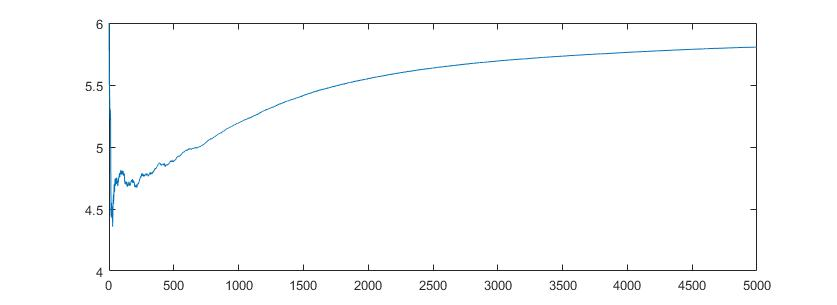
\includegraphics[width=14cm]{imagens/graf15.jpg}
\caption{Pontos acumulados em relação a reputação e o ajuste dos pontos por uma reta}
\label{fig15}
\end{figure}

O gráfico \ref{fig16} mostra que a maioria da população migrou para um perfil próximo de 1, que é significa dar peso máximo a reputação do oponente na hora de escolher a jogada.

\begin{figure}[H]
\centering
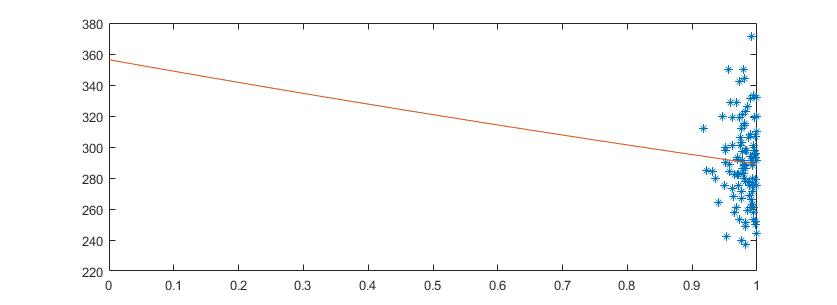
\includegraphics[width=14cm]{imagens/graf16.jpg}
\caption{Pontos acumulados em relação ao perfil e o ajuste dos pontos por uma reta}
\label{fig16}
\end{figure}

Esses resultados foram dá ultima população, a mais aperfeiçoada. Agora veremos abaixo dois gráficos que mostram a evolução da cooperação e do perfil ao longo de todas as populações. No gráfico \ref{fig17} temos o ganho médio por jogo em cada simulação, nas primeiras populações era próximo de 5, e o 5 só pode ser obtido pela matriz de pontos somando 5+0, ou seja, um cooperando e outro não, mas nas etapas seguintes esse numero foi subindo e tendendo a 6, que é obtido por 3+3, ou seja, quando ambos cooperam. No gráfico \ref{fig18} o perfil médio da população tendendo a um, ou seja, cada jogador dando prioridade máxima a reputação do seu oponente.

\begin{figure}[H]
\centering
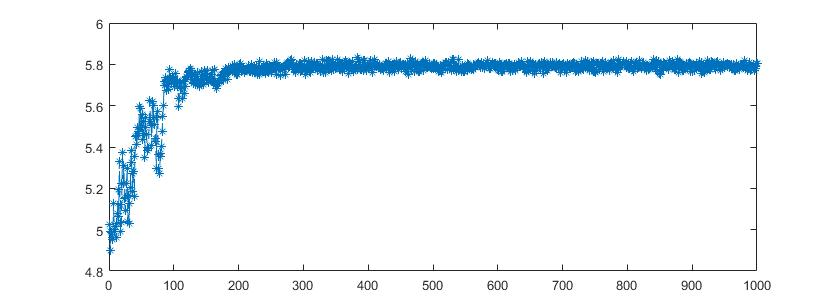
\includegraphics[width=14cm]{imagens/graf17.jpg}
\caption{Ganho médio por jogada em cada simulação.}
\label{fig17}
\end{figure}

\begin{figure}[H]
\centering
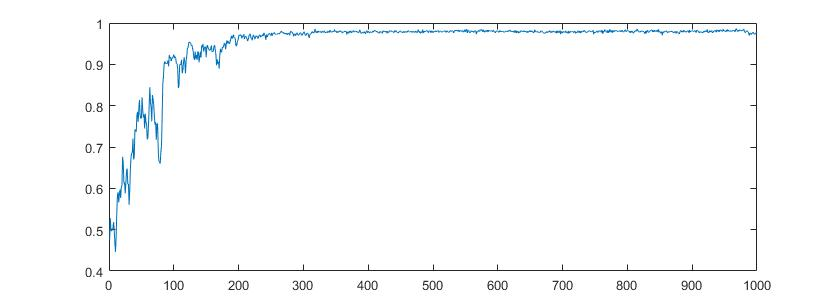
\includegraphics[width=14cm]{imagens/graf18.jpg}
\caption{Perfil médio por simulação.}
\label{fig18}
\end{figure}

\section{Aplicabilidade}

Esse modelo mostra como é possível forçar a cooperação através da reputação. Essa estratégia já é usada desde os primórdios da civilização, sempre que alguém vai negociar com alguma pessoa, primeiro ela se informa pra saber se a pessoa é confiável ou não, isso nada mais é que dar prioridade a reputação da outra pessoa.

Com a globalização e o comércio pela internet, surgiu a necessidade de pensar em métodos de fazer as pessoas cooperarem mesmo sem conhecer seu consumidor ou fornecedor, e a solução foi criar mecanismo que expõe a reputação do indivíduo para consulta. Isso viabilizou e alavancou o comercio digital. Empresas como Uber, Mercado Livre, Submarino e outras empresas de vendas virtuais, controlam seus negócios e mantem um nível de cooperação reduzindo os golpes através da reputação.

%\end{document}

%\begin{figure}[H]
%\centering
%\includegraphics[height=5cm]{Imagem.png}
%\caption{legenda}
%\label{Imagem}
%\end{figure}

%\begin{equation}\nonumber

%\end{equation}\vspace{0.1cm}

%\begin{eqnarray}

%\end{eqnarray}

%\begin{propriedade}

%\end{propriedade}

%\begin{definicao}

%\end{definicao}

%\begin{ex}

%\end{ex}

%\begin{solucao}

%\end{solucao}

%\begin{teorema}

%\end{teorema}

%\begin{demo}

%\end{demo}

%\begin{flushright}
%\begin{minipage}{7cm}
%\small
%\end{minipage}\vspace{1cm}
%\end{flushright}